\documentclass[a4paper]{article}
\usepackage[paper=a4paper,left=24mm,right=24mm,top=20mm,bottom=20mm]{geometry}

%% Language and font encodings
\usepackage[english]{babel}
%\usepackage[utf8x]{inputenc}
\usepackage{pgfgantt}
\usepackage{rotating}
%\usepackage[english, ngerman]{babel}
\usepackage{graphicx}                               % For includegraphics
\usepackage{wrapfig}                                % For wrapfig environment
\usepackage{paralist}                               % For compactitem 
\usepackage{xcolor}
\usepackage[utf8]{inputenc}
\usepackage{sectsty}
\usepackage{hyperref}
\usepackage{paralist}
\usepackage{booktabs}
\usepackage{tabu}
\usepackage[affil-it]{authblk}
\usepackage[T1]{fontenc}

%% Sets page size and margins

%% Useful packages
\usepackage{amsmath}
%\usepackage{apacite}
\usepackage[colorinlistoftodos]{todonotes}
\renewcommand\Authfont{\fontsize{14}{14.4}\selectfont}
\renewcommand\Affilfont{\fontsize{12}{14.4}\selectfont}
%\usepackage[colorlinks=true, allcolors=blue]{hyperref}
%Write the title of your project here:
\title{Differentiate Sparse Matrix with a Reversible Embeded Domain-Specific Language}
%Here goes your full name
\author{Jie Li}
\affil{Mentors: Jinguo Liu, Jiuning Chen}
\date{\today}

\begin{document}
\maketitle

\section{Summary of the Proposal}

Sparse matrices are extensively used in scientific computing, however there is no automatic differentiation package in Julia yet to handle sparse matrix operations yet. This project will utilize the reversible embedded domain-specific language NiLang.jl to differentiate sparse matrix operations by re-writing the sparse functions in Julia base in a reversible style. We will port the generated backward rules to ChainRules.jl as an extension, where ChainRules.jl is the most popular Julia package providing backward rules for automatic differentiation packages.

\section{Introduction}

Content included in \textbf{Para1}
\begin{itemize}
    \item Importance of Sparse Matrix
    \item Automatic Differentiation topic generalization
    \item Reviewing previous tools, forward AD, reverse AD and mixed AD
\end{itemize}

Content included in \textbf{Para2}
\begin{itemize}
    \item Gap between classical AD and eDSL\cite{liu2020differentiate}
    \item Outline purpose: implement AD for sparse matrix operations
    \item Summarize methods and expected outcome
    \item State the value
\end{itemize}

Content included in \textbf{Para3}  
\begin{itemize}
    \item Structure of this proposal
\end{itemize}




\section{Goal and Objectives}
\label{sec:goals}
\begin{itemize}
    \item An automatic differentiation on sparse matrix Julia package writen by NiLang
    \item Test converage above 80\%
    \item  Export chain rules into ChainRules.jl
\end{itemize} 

\section{Design and Decision Details}

\subsection{SparseCSC}
SparseCSC format for sparse matrix in julia

\subsection{Low Level Operations}
sparse matrix operation  

sparse tensor operation (needed?)

\subsection{High Level Operations}
pca-lowrank, svd-lowrank

\subsection{Export Chain Rules into ChainRules.jl}
define rules for sparse matrix

\section{Delivery, Schedule and Timeline}

\subsection{Delivery}
expectation packages

\subsection{Schedule}
ask advice from mentors

\subsection{Timeline}
 Gantt chart \cite{gantt1910work}
\vspace{0.5cm}

\noindent\resizebox{\textwidth}{!}{
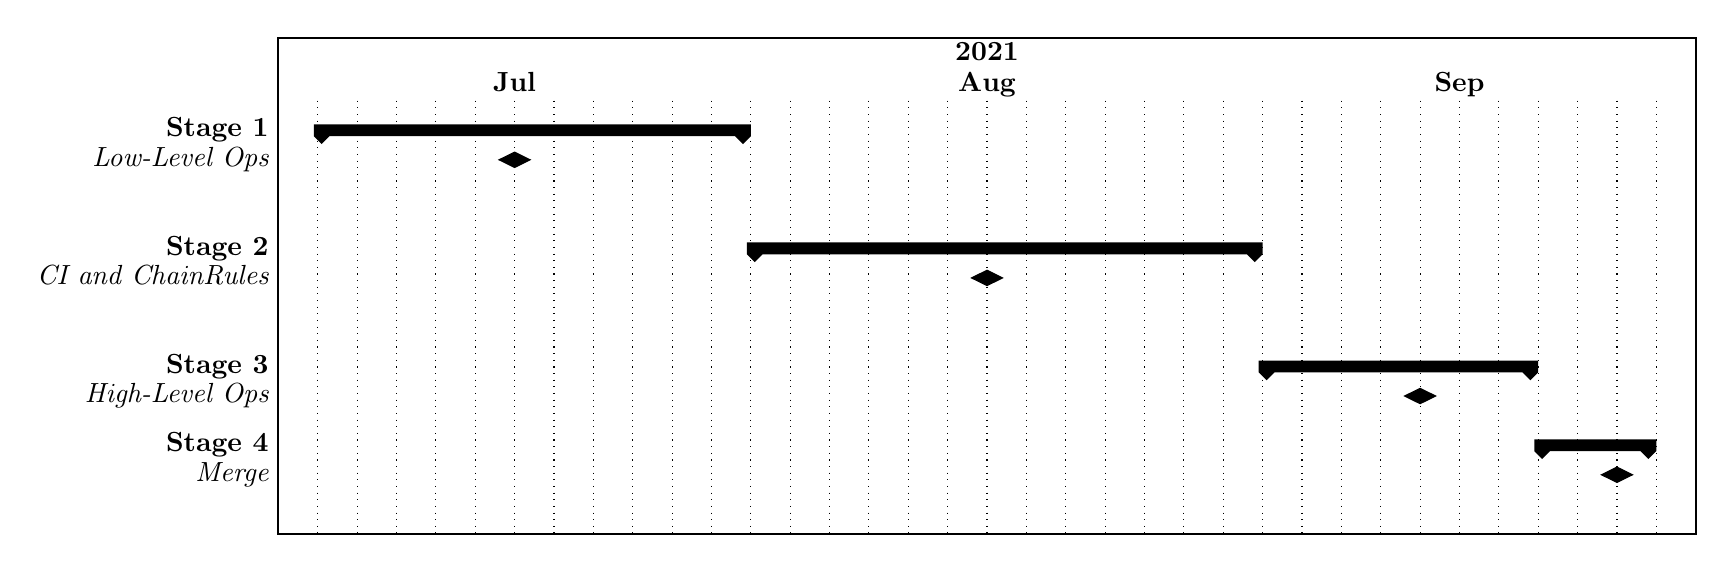
\begin{tikzpicture}[x=.5cm, y=1cm] 
\centering
        \begin{ganttchart}[%Specs
            y unit title=0.4cm,
            y unit chart=0.5cm,
            canvas/.style={fill=none, draw=black, line width=.75pt},
            vgrid,
            title label anchor/.style={below=-1.6ex},
            title left shift=.05,
            title right shift=-.05,
            title height=1,
            title/.style={fill=none},
            title label font=\bfseries,
            bar/.style={fill=barblue},
            incomplete/.style={fill=white},
            progress label text={},
            bar height=0.7,
            group right shift=0,
            group top shift=.6,
            group height=.3,
            group peaks height=.2]{1}{36}

            %labels
            \gantttitle{2021}{36}\\
            \gantttitle{Jul}{12}
            \gantttitle{Aug}{12}
            \gantttitle{Sep}{12}
            \\

            % Parameter Selection
            \ganttgroup{Stage 1}{2}{12}\\ %elem0
            %\ganttbar[progress=0]{sub-objective}{2}{18}\\
            \ganttmilestone{Low-Level Ops}{6}\\\\

            % Testing equipment
            \ganttgroup{Stage 2}{13}{25}\\ %elem0
            %\ganttbar[progress=0]{Bar}{2}{18}\\
            \ganttmilestone{CI and ChainRules}{18}\\\\

            % Testing
            \ganttgroup{Stage 3}{26}{32}\\ 
            %\ganttbar[progress=0]{Bar}{19}{35}\\
            %\ganttbar[progress=0]{Bar}{19}{35}\\
            \ganttmilestone{High-Level Ops}{29}\\
            %\ganttmilestone{Milestone}{35}\\

            % Algorithm Development
            \ganttgroup{Stage 4}{33}{35}\\
            \ganttmilestone{Merge}{34}\\ 
            %\ganttbar[progress=0]{Bar}{28}{35} \\

            %relations 
            %\ganttlink{elem2}{elem6}
            %\ganttlink{elem5}{elem6}
            %\ganttlink{elem9}{elem11}

        \end{ganttchart}
    \label{fig:Gantt2014}
\end{tikzpicture}}  




\bibliographystyle{plain}
\bibliography{refs}

\newpage
\pagestyle{empty}                                   % No pagenumbers/headers/footers

%%% Custom sectioning (sectsty package)
\sectionfont{%			                            % Change font of \section command
	\usefont{OT1}{serif}{m}{n}%		                
	\sectionrule{0pt}{0pt}{-10pt}{1pt}
}
\subsectionfont{%			                        % Change font of \subsection command
	\usefont{OT1}{serif}{m}{n}%		                
	%\sectionrule{0pt}{0pt}{-10pt}{1pt}
}

%%% Macros
\newcommand{\sepspace}{\vspace*{1em}}		        % Vertical space macro
\newcommand{\NewPart}[1]{\section*{\uppercase{#1}}}
\newcommand{\NewSubPart}[1]{\subsection*{#1}}

\newcommand{\MyName}[1]{
    \noindent
	\Huge \usefont{OT1}{serif}{eb}{n} #1 \hfill        % Name
	\par \normalsize \normalfont
}

\newcommand{\SimpleEntry}[1]{
	\noindent\hangindent=0.5cm\hangafter=0          % Indentation
	#1 \par                                         % Entry 
}

\newcommand{\TimeEntry}[4]{
    \noindent\hangindent=0.5cm\hangafter=0          % Indentation
    \parbox{3cm}{                                   % Box to align text
	    \textit{#1}                                 % Time
	}
	\textbf{#2}                                     % What
	\text{#3}                                       % Work
	\normalsize \par
}

\newcommand{\TimeEntryFocus}[5]{
    \noindent\hangindent=0.5cm\hangafter=0          % Indentation
    \parbox{3cm}{                                   % Box to align text
	    \textit{#1}                                 % Time
	}
	\textbf{#2}                                     % What
	\text{#3} \par                                  % School
	\noindent\hangindent=3.7cm\hangafter=0
	\textit{#4}                                     % Average, Focus, etc
	\normalsize \par
}

\newcommand{\TimeEntryDesc}[4]{
    \noindent\hangindent=0.5cm\hangafter=0          % Indentation
    \parbox{3cm}{                                   % Box to align text
	    \textit{#1}                                 % Time
	}
	\textbf{#2}                                     % What
	\text{#3} \par                                  % Work
	\noindent\hangindent=4cm\hangafter=0 \parbox{11cm}{\vspace{0.2em}\small #4}  % Description
	\normalsize \par
}

\newcommand{\TimeEntryFocusDesc}[5]{
    \noindent\hangindent=0.5cm\hangafter=0          % Indentation
    \parbox{3cm}{                                   % Box to align text
	    \textit{#1}                                 % Time
	}
	\textbf{#2}                                     % What
	\text{#3} \par                                  % School
	\noindent\hangindent=3.7cm\hangafter=0
	\textit{#4} \par                                  % Average, Focus, etc
	\noindent\hangindent=4cm\hangafter=0 \parbox{12cm}{\vspace{0.2em}\small #5}  % Description
	\normalsize \par
}

\newcommand{\TitleEntry}[2]{                     
	\noindent\hangindent=0.5cm\hangafter=0            % Indentation
	\parbox{3cm}{                                   % Box to align text
	    \textit{#1}
	}			                                    % Title
	#2 \par                                         % Entry	
}

\newcommand{\TitleEntryLong}[2]{                     
	\noindent\hangindent=0.5cm\hangafter=0            % Indentation
	\parbox{14cm}{                                   % Box to align text
	    \textit{#1}
	}			                                    % Title
	#2 \par                                         % Entry	
}

\MyName{Jie Li}

\sepspace

%%% Personal details--------------------------------------------------------------------------

\SimpleEntry{\textbf{Github}: \href{https://github.com/jieli-matrix}{https://github.com/jieli-matrix}}
\SimpleEntry{\textbf{Website}: \href{https://jieli-matrix.github.io/}{https://jieli-matrix.github.io/}}
\SimpleEntry{\textbf{Email}: li\_j20@fudan.edu.cn}

%%% Education---------------------------------------------------------------------------------
\NewPart{Education}

\TimeEntryFocus{9.2020 - 6.2023}
{Master of Applied Mathematics }{at Fudan University}
{Supervised by Young PI \href{https://scholar.google.com/citations?user=bLERs80AAAAJ&hl=zh-CN}{Weiyang Ding}\\
Focus on Numerical Optimization and Matrix Computation}
\sepspace

\TimeEntry{9.2016 - 7.2020}
{Bachelor of Mathematics and Applied Mathematics}{at Lanzhou University}
\sepspace


%%% Skills and Qualifications --------------------------------------------------------------
\NewPart{Skills and Qualifications}
\NewSubPart{Programming Languages}
\TitleEntry{Advanced skills}{Python, Julia, Matlab}
\TitleEntry{Basic skills}{Git, Linux, Cpp}

\NewSubPart{Languages}
\TitleEntry{Native}{Chinese}
\TitleEntry{Advanced}{English (TOEFL:94 CET-4:632 CET-6:571)}

%%% Work experience------------------------------------------------------------------------
\NewPart{internship experience}
\TimeEntryDesc{10.2019 - 12.2019}{NLP Researcher in Core Development Platform}{at \href{https://www.iflytek.com/}{iFLYTEK}}
{\begin{compactitem}
    \item Automatic Pipeline on Senior High School Math Homework 
    \item Code Implementation of  \href{https://arxiv.org/abs/1911.06557}{Multi-Label Learning with Deep Forest}
\end{compactitem}
}



%%% Skills and Qualifications --------------------------------------------------------------
\NewPart{Projects}
\TimeEntryDesc{5.2021 - now}{Lowranksvd.jl}{ \href{https://github.com/jieli-matrix/Lowranksvd.jl/tree/dev}{Lowranksvd.jl}}
{\begin{compactitem}
    \item Algorithm 4.4 from \href{https://arxiv.org/abs/0909.4061}{Halko et al.} implemented by Julia with all CI tests passing.
    \item Algorithm 5.1 from \href{https://arxiv.org/abs/0909.4061}{Halko et al.} implemented by Julia with all CI tests passing.
\end{compactitem}
}

\TimeEntryDesc{4.2020}{CPUPredict}{\href{https://github.com/VealM/CPUPredict}{CPUPredict}}
{
    Time series prediction of the CPU's usage rates.  

    This project won the third place in Elastic Cloud College Challenge held by ALibaba.
}

\NewPart{Contests}
\TimeEntryDesc{11.2020}{Brain-Inspired Intelligence Contests held by Fudan University}{\quad}{
    \textbf{Efficent information encoding and energy efficiency in E/I balanced neuronal networks}  

    Numerical Simulation for E/I balanced neuronal networks.  
      
    I won the third place in the contest. 
}



\end{document}